\documentclass{standalone}

\usepackage{tikz}
\usepackage{graphicx}
\pagestyle{empty}

% INT_AY22_L35-Fig03_Wire_approx.png

\begin{document}
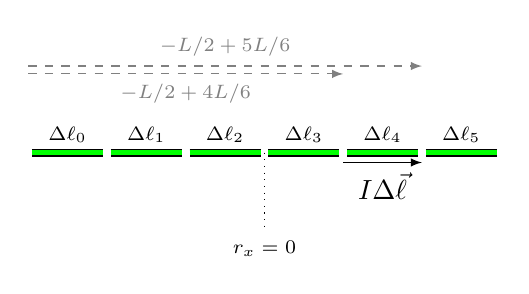
\begin{tikzpicture}[> = latex]

	% Definitions
	
	\def\L{6}		% Wire length
	\def\N{6} 		% Number of wire segments
	\def\R{1}		% Distance to observation point
	
	% Wire segments
	
	\foreach \n in {0, 1, ..., 5}
		\draw [double = green, double distance = 2 pt] ({(\n + 0.05) * \L / \N}, 0) -- node [above, font = \scriptsize] {$\Delta \ell_\n$} ({(\n + 0.95) * \L / \N}, 0);

	% Left, right length vectors

	\draw [dashed, gray, ->] (0, \R) -- node [below, font = \scriptsize] {$-L/2 + 4L / 6$} ({4 * \L / \N}, \R);
	\draw [dashed, gray, ->] (0, 1.1 * \R) -- node [above, font = \scriptsize] {$-L/2 + 5L / 6$} ({5 * \L / \N}, 1.1 * \R);
	
	% Length vector
	
	\draw [->] ({(\N - 2) * \L / \N}, -0.125) -- node [below] {$I \Delta {\vec \ell}$} ({(\N - 1) * \L / \N}, -0.125);

	% r_x = 0 line

	\draw [dotted] ({\L/ 2}, 0) -- ({\L / 2}, -\R) node [below, font = \scriptsize] {$r_x = 0$};

\end{tikzpicture}
\end{document}